\documentclass{UTNetLab}

\title{Multicast and Realtime Service}
\newcommand{\difficulty}{10}
\newcommand\reference{
   S. Panwar, S. Mao, J.-dong Ryoo, and Y. Li, “Multicast and realtime service,” in TCP/IP Essentials: A Lab-Based Approach, Cambridge: Cambridge University Press, 2004, pp. 134–158.
}

\begin{document}
	\section*{Objectives}
	\begin{itemize}
		\item Multicast addressing.
		\item Multicast group management.
		\item Multicast routing: configuring a multicast router.
		\item [-] Realtime video streaming using the \textbf{vlc}.
		\item [-] Protocols supporting realtime streaming: RTP/RTCP and RTSP.
		\item [-] Analyzing captured RTP/RTCP packets using \textbf{wireshark}.
	\end{itemize}
\part{Simple Multicast Exercises\label{sec:simple-multicast}}
    For all the exercises in this section, the network topology is given in \hyperref[fig:1.3]{Figure~1.3}, where all the hosts are connected to a single network segment using their default IP addresses, i.e.\ from 128.238.66.100 to 128.238.66.107.
    
    \begin{minipage}{0.48\textwidth}
        \begin{flushleft}
            \begin{table}[H]
                \caption{The IP addresses of the hosts (Table~1.2)}
                \label{tab:1.2}
                \centering
                \begin{tabular}{ c c c }
                    \hline \hline
                    Host & IP Address & Subnet Mask \\
                    \hline 
                    h0 & 128.238.66.100 & 255.255.255.0 \\
                    h1 & 128.238.66.101 & 255.255.255.0 \\
                    h2 & 128.238.66.102 & 255.255.255.0 \\
                    h3 & 128.238.66.103 & 255.255.255.0 \\
                    h4 & 128.238.66.104 & 255.255.255.0 \\
                    h5 & 128.238.66.105 & 255.255.255.0 \\
                    h6 & 128.238.66.106 & 255.255.255.0 \\
                    h7 & 128.238.66.107 & 255.255.255.0 \\
                    \hline \hline
                    \end{tabular}
            \end{table}
        \end{flushleft}
    \end{minipage}
    \begin{minipage}{0.48\textwidth}
        \begin{flushright}
            \begin{figure}[H]
                \centering
                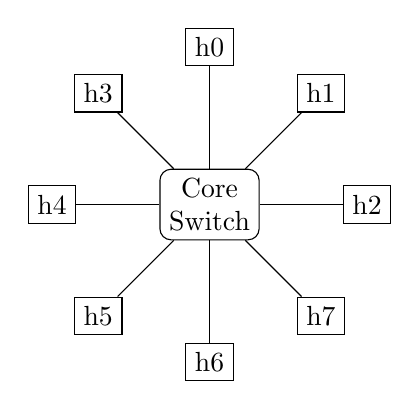
\begin{tikzpicture}
                    \node[draw,rounded corners,align=center] (s) at (0,0) {Core\\Switch};
                    \node[draw] (h0) at (0,2){h0};
                    \node[draw] (h1) at ({sqrt(2)},{sqrt(2)}){h1};
                    \node[draw] (h2) at (2,0){h2};
                    \node[draw] (h3) at (-{sqrt(2)},{sqrt(2)}){h3};
                    \node[draw] (h4) at (-2,0){h4};
                    \node[draw] (h5) at (-{sqrt(2)},-{sqrt(2)}){h5};
                    \node[draw] (h6) at (0,-2){h6};
                    \node[draw] (h7) at ({sqrt(2)},-{sqrt(2)}){h7};
                
                    \draw (h0) -- (s);
                    \draw (h1) -- (s);
                    \draw (h2) -- (s);
                    \draw (h3) -- (s);
                    \draw (h4) -- (s);
                    \draw (h5) -- (s);
                    \draw (h6) -- (s);
                    \draw (h7) -- (s);
                \end{tikzpicture}
                \caption{A single segment network (Figure~1.3)}
                \label{fig:1.3}
            \end{figure}
        \end{flushright}
    \end{minipage}

\section{Linux Multicast Routing Table\label{sec:rt}}
\label{sec:linux-multicast-routing}
    Execute the following command to display the routing table of one host (for example \textit{h0}).

    \fcolorbox{blue}{red!10}{{h\textsubscript{0}}'s Console}
    \lstset{backgroundcolor=\color{red!10}}
    \begin{lstlisting}
	netstat -rn
    \end{lstlisting}
    
    \textbf{Note: }If there is no entry for the 224.0.0.0 subnet, you need to provide a default route for multicast traffic, by:
    \footnote{This command can be appended to the \path{/etc/rc.local} file, so that it will be executed automatically when the system bootstraps.
    Each time when the network interface is brought down and up again by the \lstinline{ifconfig} command, you may need to run the \lstinline{route} command to re-insert the multicast routing entry.}

 \fcolorbox{blue}{green!10}{{h\textsubscript{i}}'s Console , i $\in$ \{0,1,...,7\}}
    \lstset{backgroundcolor=\color{green!10}}
    \begin{lstlisting}[emph=eth0]
	route add -net 224.0.0.0 netmask 240.0.0.0 dev eth1
    \end{lstlisting}
    
    Then, run the first command, \textit{i.e.} \lstinline{netstat -rn}. Save the new routing table.
    
    \fcolorbox{blue}{red!10}{{h\textsubscript{0}}'s Console}
    \lstset{backgroundcolor=\color{red!10}}
    \begin{lstlisting}
    netstat -rn
    \end{lstlisting}
    
    \begin{report}
        \item Submit the routing table you saved.
    \end{report}

\section{Multicast Membership}
    Execute the following command to show the multicast group memberships for all the interfaces in your host (for example \textit{h0}).

    \fcolorbox{blue}{red!10}{{h\textsubscript{0}}'s Console}
    \lstset{backgroundcolor=\color{red!10}}
    \begin{lstlisting}
	netstat -g
    \end{lstlisting}
    
    \begin{report}
        \item How many multicast groups did the interface belong to? What were the groups? Explain the meaning of the group IDs.
    \end{report}

\section{Multicast \texttt{ping}}
%     Set all hosts \textit{h0}, \textit{h2}, \textit{h4} and \textit{h6} to replry linux multicast routing in all the hosts:
%     \begin{lstlisting}[emph={eth0}]
% echo 0 > /proc/sys/net/ipv4/icmp_echo_ignore_broadcasts
%     \end{lstlisting}

    Execute the following command on \textit{h1}:

    \fcolorbox{blue}{red!10}{{h\textsubscript{1}}'s Console}
    \lstset{backgroundcolor=\color{red!10}}
    \begin{lstlisting}
	ping 224.0.0.1
    \end{lstlisting}
Examine the \lstinline{ping} output to see which hosts reply.

Ping a broadcast address using:

    \fcolorbox{blue}{red!10}{{h\textsubscript{1}}'s Console}
    \lstset{backgroundcolor=\color{red!10}}
    \begin{lstlisting}
	ping -b 128.238.66.255
    \end{lstlisting}
    Examine the \lstinline{ping} output to see which hosts reply.

\textbf{Note: }You can see and change the broadcast ping replay state of a host using the following commands (in the PNETLab figure we've set them for you):
\lstset{backgroundcolor=\color{green!10}}
\begin{lstlisting}[emph=eth0]
    # see (read) kernel value
    cat /proc/sys/net/ipv4/icmp_echo_ignore_broadcasts
    sysctl net.ipv4.icmp_echo_ignore_broadcasts
    
    # set (write) kernel value
    # 0 for disable and 1 for enable the kernel feature
    echo 0 > /proc/sys/net/ipv4/icmp_echo_ignore_broadcasts
    sysctl -w net.ipv4.icmp_echo_ignore_broadcasts=0
    
    # add to sysctl.conf file to load configuration on boot time
    echo "net.ipv4.icmp_echo_ignore_broadcasts = 0" >> /etc/sysctl.conf
\end{lstlisting}
    
    \begin{report}
        \item Which hosts replied when the multicast address was pinged?
            Which hosts replied when the broadcast address was pinged?
            Verify you answers with hosts config \path{/proc/sys/net/ipv4/icmp_echo_ignore_broadcasts}.

        \item In each case, was there a reply from \textit{h0} and \textit{h1}?
    \end{report}

\section{Multicast vs Unicast\label{sec:multicast-vs-unicast}}
    On \textit{h1} execute \lstinline{wireshark} and \lstinline{tcpdump ether multicast -n -nn -e} to capture an Ethernet unicast frame, an Ethernet multicast frame, and an Ethernet broadcast frame.

    \fcolorbox{blue}{lime!30}{{h\textsubscript{1}'s Wireshark}}
    \lstset{backgroundcolor=\color{lime!30}}
    \begin{lstlisting}
    Run wireshark on eth1          # to capture all packets
    \end{lstlisting}
 
   \fcolorbox{blue}{red!10}{{h\textsubscript{1}}'s Console}
 \lstset{backgroundcolor=\color{red!10}}
 \begin{lstlisting}[emph={your-host, remote-host}]
 	tcpdump ether multicast -n -nn -e -i eth1			# to capture just multicast and broadcast packets
 \end{lstlisting}
 
To generate an Ethernet unicast frame, run below command:

 \fcolorbox{blue}{red!10}{{h\textsubscript{0}}'s Console}
\lstset{backgroundcolor=\color{red!10}}
\begin{lstlisting}[emph={your-host, remote-host}]
	socket -i -u -n1 128.238.66.101 echo
\end{lstlisting}

   Execute the following command in \textit{h0} to generate an Ethernet multicast frame:
   
    \fcolorbox{blue}{red!10}{{h\textsubscript{0}}'s Console}
    \lstset{backgroundcolor=\color{red!10}}
    \begin{lstlisting}[emph={your-host, remote-host}]
	socket -i -u -n1 230.11.111.10 2000
    \end{lstlisting}

    Generate another Ethernet multicast frame, but with a different group address of {232.139.111.15}, e.g.:

    \fcolorbox{blue}{red!10}{{h\textsubscript{0}}'s Console}
    \lstset{backgroundcolor=\color{red!10}}
    \begin{lstlisting}[emph={your-host, remote-host}]
    socket -i -u -n1 232.139.111.15 2000
    \end{lstlisting}


    To generate an Ethernet broadcast frame, you may \lstinline{ping} a remote host from \textit{h0} that has no entry in the ARP table of your host, e.g.\ \textit{h5}.
    \footnote{You can see ARP table by \lstinline{arp -a} delete a cached ARP entry by \lstinline[emph={ip}]{arp -d ip}.}

    \fcolorbox{blue}{red!10}{{h\textsubscript{0}}'s Console}
    \lstset{backgroundcolor=\color{red!10}}
    \begin{lstlisting}
	ping 128.238.66.105
    \end{lstlisting}
    Recall that the ARP request is broadcast.%

    Save the frames captured for the lab report.

    \begin{report}
        \item Compare the source and destination MAC addresses of the frames you captured.

        \item Use one of the multicast frames captured to explain how a multicast group address is mapped to a multicast MAC address.
            For the two multicast frames captured, do they have the same destination MAC address?
            Why?
    \end{report}

\section{Simple UDP Multicast Client and Server}

    % \lstinline{netspy} and \lstinline{netspyd} programs are located in \textit{code} directory for \textit{netlab} user.
    
%     You can go there by the following command:
%     \begin{lstlisting}
% cd /home/netlab/code
%     \end{lstlisting}
    
%     You can compile source codes, if needed, by:
%     \begin{lstlisting}[emph={fileName, outputName}]
% gcc fileName -o outputName
%     \end{lstlisting}
\textbf{Note: }Go to \textit{code} directory for \textit{netlab} user at \textit{/home/netlab/code} with \textit{cd} command.
You can compile source code with \lstinline[emph={$fileName, $outputName}]{gcc $fileName -o $outputName}{}.

    Start the multicast client \lstinline{netspy} in the background of all hosts, by executing:%
    \footnote{If you get \textit{Netspy : cannot join multicast group `224.111.111.111'}, add route for the groups as described in \autoref{sec:rt}.}

    \fcolorbox{blue}{blue!10}{{h\textsubscript{i}}'s Console, i $\in$ \{0,1,...,7\}}
    \lstset{backgroundcolor=\color{blue!10}}
    \begin{lstlisting}
	/home/netlab/code/netspy 224.111.111.111 1500 &
    \end{lstlisting}
    
    Then, start the multicast sender \lstinline{netspyd} on \textit{h0}, by executing:

    \fcolorbox{blue}{red!10}{{h\textsubscript{0}}'s Console}
    \lstset{backgroundcolor=\color{red!10}}
    \begin{lstlisting}
	/home/netlab/code/netspyd 224.111.111.111 1500 1
    \end{lstlisting}
    
    Now, execute \lstinline{tcpdump ip multicast -i eth1} or \lstinline{wireshark} on every host to capture multicast IP datagrams. For example, in \textit{h1}'s Console run the below command:

 \fcolorbox{blue}{red!10}{{h\textsubscript{1}}'s Console}
\lstset{backgroundcolor=\color{red!10}}
\begin{lstlisting}
	tcpdump ip multicast -i eth1			# or run wireshark
\end{lstlisting}

%     Start \textit{ssh} service on \textit{h0} by:
%     \begin{lstlisting}
% service ssh start
%     \end{lstlisting}

Login to \textit{h0} from a remote machine, e.g.\ \textit{h6}, using \lstinline{telnet}

    \fcolorbox{blue}{red!10}{{h\textsubscript{6}}'s Console}
    \lstset{backgroundcolor=\color{red!10}}
    \begin{lstlisting}
	telnet 128.238.66.100
    \end{lstlisting}
    Use \texttt{netlab} as username and password.

    Save the captured multicast datagram sent by \lstinline{netspyd} and exit the \lstinline{telnet} session.

    \begin{report}
        \item From the \lstinline{tcpdump} output, how many messages are sent by \lstinline{netspyd} when a new user logged in to \textit{h0}?
            From the \lstinline{netspy} outputs on all the hosts, how many copies of the message are received in total?

        \item Did \textit{h0}, where the multicast sender, \lstinline{netspyd}, was running, receive the multicast datagram?
            Why?
            If yes, through which interface did \textit{h0} receive this datagram?
    \end{report}

\section{\texttt{ping} Replay}
    % Enable broadcast ping replay by: \lstinline{echo 0 > /proc/sys/net/ipv4/icmp_echo_ignore_broadcasts} on all hosts.
    Keep the \lstinline{netspy} and the \lstinline{wireshark} (on \textit{h6}) programs running.
    Execute the following command from \textit{h6}:

    \fcolorbox{blue}{lime!30}{{h\textsubscript{6}'s Wireshark}}
    \lstset{backgroundcolor=\color{lime!30}}
    \begin{lstlisting}
    Run wireshark on eth1          # or use tcpdump
    \end{lstlisting}

    \fcolorbox{blue}{red!10}{{h\textsubscript{6}}'s Console}
    \lstset{backgroundcolor=\color{red!10}}
    \begin{lstlisting}
	ping 224.111.111.111
    \end{lstlisting}
    Examine the \lstinline{wireshark} and \lstinline{ping} outputs to see which hosts replied.

    Terminate the \lstinline{netspy} client programs on several hosts, e.g.\ \textit{h2}, \textit{h3} and \textit{h5} (first use \lstinline{fg} command to bring them to foreground and then use Ctrl+C to terminate them).
    Execute the \lstinline{ping} command again.

    Again, examine the \lstinline{wireshark} and \lstinline{ping} outputs (on \textit{h6}) to see which hosts replied.

\part{IGMP Exercises}\label{sec:igmp}
    In the following exercises, use four hosts and one router.
    The network topology is given in \hyperref[fig:7.13]{Figure~7.13}, and the corresponding host IP addresses and router IP addresses are given in \hyperref[tab:7.2]{Table~7.2} and \hyperref[tab:7.3]{Table~7.3}, respectively.

    \begin{table}[H]
        \caption{Hosts IP addresses for \hyperref[fig:7.13]{Figure~7.13} (Table~7.2)}
        \label{tab:7.2}
        \centering
        \begin{tabular}{ *3c }
            \hline \hline
            Name & IP Address \\
            \hline
                h1 & 128.238.63.101/24 \\
                h2 & 128.238.63.102/24 \\
                h3 & 128.238.64.103/24 \\
                h4 & 128.238.64.104/24 \\
            \hline \hline
            \end{tabular}
    \end{table}

    \begin{table}[H]
        \caption{Router IP addresses for \hyperref[fig:7.13]{Figure~7.13} (Table~7.3)}
        \label{tab:7.3}
        \centering
        \begin{tabular}{ *3c }
            \hline \hline
            Host & f0/0 & f1/0 \\
            \hline
            router & 128.238.63.3/24 & 128.238.64.3/24 \\
            \hline \hline
            \end{tabular}
    \end{table}

    \begin{figure}[H]
        \centering
        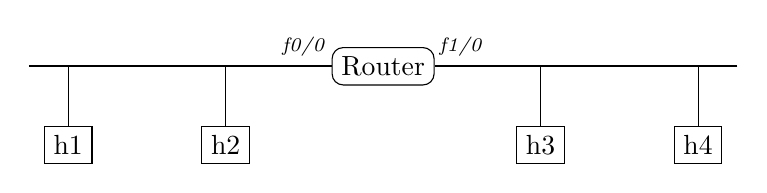
\begin{tikzpicture}
            \node[draw] (h1) at (-4,-1){h1};
            \node[draw] (h2) at (-2,-1){h2};
            \node[draw,rounded corners] (router) at (0,0){Router};
            \node[draw] (h3) at (2,-1){h3};
            \node[draw] (h4) at (4,-1){h4};
        
            \draw (h1) -- (-4,0);
            \draw (h2) -- (-2,0);
            \draw (h3) -- (2,0);
            \draw (h4) -- (4,0);
            \draw[thick] (4.5,0) -- (router);
            \draw[thick] (-4.5,0) -- (router);
            \draw (router) +(1,0.25) node[align=right] {\scriptsize\textit{f1/0}};
            \draw (router) +(-1,0.25) node[align=left] {\scriptsize\textit{f0/0}};
        \end{tikzpicture}
        \caption{The network topology for \nameref{sec:igmp} (Figure~7.13)}
        \label{fig:7.13}
    \end{figure}

%     Enable linux multicast routing in all the hosts (see \autoref{sec:simple-multicast}):
%     \begin{lstlisting}[emph={eth0}]
% route add -net 224.0.0.0 netmask 240.0.0.0 dev eth0
% route add -net 128.238.0.0/16 dev eth0
% echo 0 > /proc/sys/net/ipv4/icmp_echo_ignore_broadcasts
%     \end{lstlisting}

    You can use prepared topology as described in \autoref{sec:simple-multicast}.

\section{Configuring Router}
\label{sec:config-router}
    Connect the hosts and the route in your group as shown in \hyperref[fig:7.13]{Figure~7.13}.
    % Set the IP address of your host as given in \hyperref[tab:7.2]{Table~7.2}.
    % Note that the IP addresses of the router interfaces are the same as their default IP addresses.
    % ip address 128.238.63.3 255.255.255.0
    % ip address 128.238.64.3 255.255.255.0
    % no shutdown
    
    Login to the router and run \lstinline{ip multicast-routing} to enable multicast routing in the \textit{Global Configuration} mode (you may need to use the \lstinline{enable} command first).
    Then, enable the PIM protocol on each interface, by running \lstinline{ip pim dense-mode} in the \textit{Interface Configuration} mode.
    Now the router is enabled to do multicast routing using PIM.

    \fcolorbox{blue}{yellow!10}{{R's Console}}
    \lstset{backgroundcolor=\color{yellow!10}}
    \begin{lstlisting}[language=cisco]
	R# conf term
    R(config)# ip multicast-routing
    R(config)# int f0/0
    R(config-if)# ip pim dense-mode
    R(config-if)# exit
    R(config)# int f1/0
    R(config-if)# ip pim dense-mode
    R(config-if)# end
    \end{lstlisting}

    Login to the router, execute the following commands in the \textit{Privileged EXEC} mode:

    \fcolorbox{blue}{yellow!10}{{R's Console}}
    \lstset{backgroundcolor=\color{yellow!10}}
    \begin{lstlisting}[language=cisco]
	R# show ip igmp interface
	R# show ip igmp group
    \end{lstlisting}

   Examine the multicast group memberships currently recorded in the router and the configurations of the router interfaces.


\section{Multicast Message}
    Enable linux multicast routing in all the hosts (see \autoref{sec:linux-multicast-routing}).
    
    \textbf{Note:} Run the below command to enable Linux multicast routing:
    
     \fcolorbox{blue}{green!10}{{h\textsubscript{i}}'s Console , i $\in$ \{1,2,3,4\}}
    \lstset{backgroundcolor=\color{green!10}}
    \begin{lstlisting}[emph=eth0]
    route add -net 224.0.0.0 netmask 240.0.0.0 dev eth1
    \end{lstlisting}

    Start the \lstinline{netspy} client in the background of all hosts, using:

    \fcolorbox{blue}{blue!10}{{h\textsubscript{i}}'s Console , i $\in$ \{1,2,3,4\}}
    \lstset{backgroundcolor=\color{blue!10}}
    \begin{lstlisting}
	/home/netlab/code/netspy 224.111.111.111 1500 &
    \end{lstlisting}
    Start \lstinline{netspy} server on \textit{h1}, by using:

    \fcolorbox{blue}{red!10}{{h\textsubscript{1}}'s Console}
    \lstset{backgroundcolor=\color{red!10}}
    \begin{lstlisting}
	/home/netlab/code/netspyd 224.111.111.111 1500 16
    \end{lstlisting}
    
    Login to the router.
    Run the following commands in the \textit{Privileged EXEC} mode again to examine the current membership records:

    \fcolorbox{blue}{yellow!10}{{R's Console}}
    \lstset{backgroundcolor=\color{yellow!10}}
    \begin{lstlisting}[language=cisco]
	R# show ip igmp interface
	R# show ip igmp group
    \end{lstlisting}

Try if you can \lstinline{ping} a host on the other side of the router.
(e.g.\ \lstinline{ping} \textit{h4} from \textit{h2})?

    \fcolorbox{blue}{red!10}{{h\textsubscript{2}}'s Console}
    \lstset{backgroundcolor=\color{red!10}}
    \begin{lstlisting}
	ping 128.238.64.104
    \end{lstlisting}

Login to \textit{h1} from the \textit{h2} in your group, using  \lstinline{telnet}, then logout. (Use \texttt{netlab} as username and password). See if the multicast messages sent by \lstinline{netspyd} reach the other side of the router.

    \fcolorbox{blue}{red!10}{{h\textsubscript{2}}'s Console}
    \lstset{backgroundcolor=\color{red!10}}
    \begin{lstlisting}
	telnet 128.238.63.101
    \end{lstlisting}
    
% Default route has been already added in topology
%     Add \textit{route} for \textbf{other subnet} to your host and try \lstinline{ping} again:
%     \begin{lstlisting}[emph={eth0}]
% route add -net 128.238.64.0/24 dev eth0  # on h1 & h2
% route add -net 128.238.63.0/24 dev eth0  # on h3 & h4
%     \end{lstlisting}
%     Now, login to \textit{h1} from \textit{h2} in your group via \lstinline{telnet}, then logout.
    % Check if multicast messages sent by \lstinline{netspyd} reach the other side of the router.
    
    \begin{report}
        \item Can you ping a host on the other side of the router?
            Will the router forward a multicast IP datagram to the other side? Justify your answers.
    \end{report}

\section{IGMP Types}
    Execute \lstinline{tcpdump} or \lstinline{wireshark}\footnote{If you have trouble in getting packets using \lstinline{wireshark}, try \lstinline{tcpdump}.} in one console to capture IGMP messages.

    \fcolorbox{blue}{red!10}{{h\textsubscript{1}}'s Console}
    \lstset{backgroundcolor=\color{red!10}}
    \begin{lstlisting}[emph={eth0}]
	tcpdump ip multicast -v -i eth1            # or run wireshark
    \end{lstlisting}
    When you see \textbf{six or more IGMP queries} in the \lstinline{tcpdump} output, terminate \lstinline{tcpdump} program.

    Analyze the IGMP messages you captured.
    Print and save two different IGMP messages.

    Repeat the above experiment.
    Terminate \lstinline{netspy} on \textit{h2} and \textit{h4}.
    Terminate the \lstinline{tcpdump} programs and analyze the IGMP leave message you captured.
    
    \begin{report}
        \item What is the value of the Time-to-Live (TTL) field for the IGMP messages?
            Why do we not set the TTL to a larger number?

        \item What is the default frequency at which the router sends IGMP queries?
    \end{report}

\section{Router Join to Multicast-Group}
    Login to the router.
    See if you can make a router interface (e.g.\ \textit{ethernet0}) join a multicast group of 224.0.0.2, using:

    \fcolorbox{blue}{yellow!10}{{R's Console}}
    \lstset{backgroundcolor=\color{yellow!10}}
    \begin{lstlisting}[language={cisco}]
	R# conf term
    R(config)# ip multicast-routing
    R(config)# interface f0/0
    R(config-if)# ip igmp join-group 224.0.0.2
    R(config-if)# exit
    R(config)# end
    \end{lstlisting}
    
    \begin{report}
        \item Explain why the above command fails.
    \end{report}

\clearpage
\begin{appendices}

\section{Configuring a Multicast Router}
    The \lstinline[language={cisco}]{no} form of this command cancels the group membership.
    \begin{subappendices}
\subsection{Configuring IGMP}

    \lstset{backgroundcolor=\color{red!10}}
    \begin{lstlisting}[language={cisco}, emph={group-address, new-value-in-seconds}]
R1(config)# ip igmp join-group group-address
R1(config)# no ip igmp join-group group-address
R1(config)# ip igmp query-interval new-value-in-seconds
R1(config)# no ip igmp query-interval
show ip igmp groups     ! Displays the multicast groups in the attached networks.
show ip igmp interface  ! Displays multicast related information on a router interface.
debug ip igmp           ! Displays IGMP packets received and transmitted.
    \end{lstlisting}

\subsection{Configuring Multicast Routing}

    \lstset{backgroundcolor=\color{red!10}}
    \begin{lstlisting}[language={cisco}]
R1(config)# ip multicast-routing
R1(config)# no ip multicast-routing
R1(config)# ip pim [dense-mode | sparse-mode | dense-sparse-mode].
show ip mroute          ! Displays the multicast routing table.
show ip mroute summary  ! Displays a one-line summary for each entry in the multicast routing table.
show ip mroute count    ! Displays multicast statistics.
show ip dvmrp route     ! Displays the DVMRP routing table.
show ip pim neighbor    ! Lists PIM neighbors discovered by the router.
show ip pim interface   ! Displays router interface configurations.
    \end{lstlisting}

\subsection{Cisco~IOS Multicast Diagnostic Tools}

    \lstset{backgroundcolor=\color{red!10}}
    \begin{lstlisting}[language={cisco}]
mtrace
mrinfo
mstat
ping
    \end{lstlisting}
    
\end{subappendices}

\section{Wikipedia}
    You can reed more about multicast address in \href{https://en.wikipedia.org/wiki/Multicast_address}{wikipedia}.

\end{appendices}


\end{document}
